\documentclass[]{article}

% Imported Packages
%------------------------------------------------------------------------------
\usepackage{amssymb}
\usepackage{amstext}
\usepackage{amsthm}
\usepackage{amsmath}
\usepackage{enumerate}
% \usepackage{enumitem}
\usepackage{fancyhdr}
\usepackage[margin=1in]{geometry}
\usepackage{graphicx}
%\usepackage{extarrows}
%\usepackage{setspace}
%\usepackage{xcolor}
\usepackage{color}
\usepackage{longtable}
\usepackage{booktabs}
\usepackage{float}
\usepackage{tikz,lipsum,lmodern}
\usepackage[most]{tcolorbox}
\usepackage{tabularx}
% \usepackage{biblatex}
\usepackage[backend=biber,style=ieee]{biblatex} % Ensure 'style=ieee' is set
\addbibresource{references.bib} % Add your bibliography file
%------------------------------------------------------------------------------

% Header and Footer
%------------------------------------------------------------------------------
\pagestyle{plain}  
\renewcommand\headrulewidth{0.4pt}                                      
\renewcommand\footrulewidth{0.4pt}                                    
%------------------------------------------------------------------------------

% Title Details
%------------------------------------------------------------------------------
\title{Deliverable \#2: High-Level Architectural Design}
\author{SE 3A04: Software Design II -- Large System Design}
\date{}
                      

% BOX DEFINITION
% -----------------------------------------------------------------------------
\newtcolorbox{cards}[1][]{%
    enhanced,breakable,
    colframe=black,
    colback=white,
    arc=1mm,
    outer arc=1mm,
    % attach boxed title to top center={yshift=-4mm},
    boxed title style={size=small,colback=black!10!white,boxsep=2.4mm,left=0mm,right=0mm},
    coltitle=black!70!black,
    fonttitle=\bfseries\large,    
    boxsep=1mm,
    left=0mm,
    right=0mm,
    before={\noindent},
    segmentation style={solid, black!100},
    title=#1%
}
% \newcommand{\crc}{
% \begin{cards}[]
%     \textbf{Class Name:} SomeClassName
%     % \medskip % Adds spacing
%     % \noindent\rule{\linewidth}{0.4pt} % Full-width horizontal line
%     % \medskip
%     \tcbline
%     \begin{tabular}{p{0.45\linewidth} | p{0.45\linewidth}}
%         \textbf{Responsibility:}& 
%         \textbf{Collaborator:}\\
%         % \hline % Horizontal line inside the table
%     \end{tabular}
%     \tcbline
%     \begin{tabular}{p{0.45\linewidth} | p{0.45\linewidth}}
%         \begin{itemize}
%             \item 
%         \end{itemize}
%         &
%         \begin{itemize}
%             \item 
%         \end{itemize}
%     \end{tabular}
% \end{cards}
% }

%------------------------------------------------------------------------------

% Document
%------------------------------------------------------------------------------
\begin{document}

\maketitle	
\noindent{\bf Tutorial Number:} T02\\
{\bf Group Number:} Group 5 \\
{\bf Group Members:} 
\begin{itemize}
	\item Andy Huynh (Leader)
	\item Gurmanjot Minhas
	\item Sarah Dorfman
	\item Ke Ma
	\item Cheukman Zhou
\end{itemize}

\newpage

% SECTION 1 
\section{Introduction}
\label{sec:introduction}
% Begin Section


\subsection{Purpose}
\label{sub:purpose}
% Begin SubSection
The purpose of the \textbf{SRS} is to serve as an outline of \textbf{Languify} for the developers, clients, and other stakeholders. It provides these stakeholders with a broad understanding of the requirements and design considerations. Section 1 establishes the scope of the product and defines any terms or references that will be mentioned in the rest of the document.
% End SubSection


\subsection{Scope}
\label{sub:scope}
% Begin SubSection
The product is a mobile app called \textbf{Languify} that takes an input from the user and identifies the language. 
A User Interface takes in a written text input in the form of a PDF document, image, or typed text. 
The input is then sent to a backend server called the Expert Manager that communicates with 3 different \textbf{experts} who specify what language they believe the input is. 
The User Interface will interact with the Controller, which interacts with two components.
These components are the data structure Language Info, which stores facts about different languages, and Layout Rules, which acts as a knowledge source on how to lay out the data.\\ \\
The \textbf{experts} are skilled at specific scripts or categories of script and identifying languages from those groups. The first expert identifies languages that use the Latin script, such as English and German. 
The second expert specifies in languages that use the Arabic script, such as Arabic and Urdu \cite{Britannica2025_WritingSystems}. The third expert specializes in languages that have a unique script, such as Korean which is the only widely spoken language that uses Hangul \cite{Britannica2025_Hangul}. \\ \\
The product only identifies languages that use Latin, Arabic, and unique scripts. It will only identify the 100 most spoken languages \cite{Ethnologue2025}. It does not distinguish between different dialects. As an innovative feature, the app displays some general information about the identified language, such as the number of speakers and some common phrases.\\ \\
The application is useful for people who are frequently exposed to languages they do not know. This is primarily for people who live in diverse regions or travellers. It is great for those who are curious about other cultures and may want to know some basic information to use. It encourages this curiosity and allows users to connect across cultural barriers. The overall goal is to make this product as accessible as possible.
% End SubSection


\subsection{Definitions, Acronyms, and Abbreviations}
\label{sub:definitions_acronyms_and_abbreviations}
% Begin SubSection
\begin{itemize}
	\item \textbf{AODA} – Accessibility for Ontarians with Disabilities Act
	\item \textbf{API} – Application Programming Interface
	\item \textbf{ISO} – International Organization for Standardization
	\item \textbf{Languify} – The name of the application that users shall recognize.
	\item \textbf{MVP} – The minimal viable product, which is a basic and usable version of the product. 
	\item \textbf{PIPEDA} – Personal Information Protection and Electronic Documents Act
	\item \textbf{SRS} – The software requirements specification, which is this document.
	\item \textbf{Agents/Experts} – Knowledge sources that help validate the correct language
\end{itemize}
% End SubSection


\subsection{References}
\label{sub:references}
% Begin SubSection
% \begin{itemize}
\printbibliography
% \bibliographystyle{IEEEtran}
% \bibliography{references}
% End SubSection


\subsection{Overview}
\label{sub:overview}
% Begin SubSection
The remainder of this document delves further into further details about the requirements specification. Section 2 is the overall product description and provides users with a general understanding of this product. This section discusses the product perspective, product functions, user characteristics, constraints, assumptions and dependencies, and apportioning of requirements. Section 3 provides a use case diagram that demonstrates how users will interact with the application. Section 4 supplements Section 3 by going into detail about functional requirements. This section also details all the main business events and viewpoints. Finally, Section 5 lists non-functional requirements and justifies their inclusion.
% End SubSection

% End Section


% SECTION 2
\section{Overall Product Description}
\label{sec:overall_description}

% Begin Section


% \begin{figure}[H]
% 	% 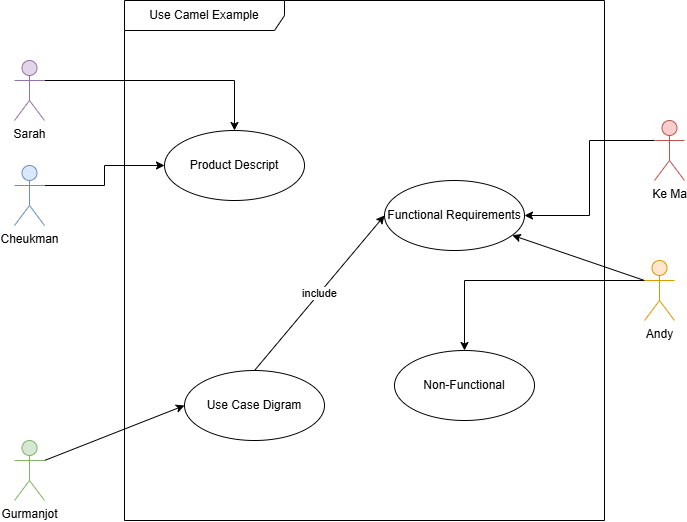
\includegraphics[width=\linewidth]{Example_Use_Case.png}
% 	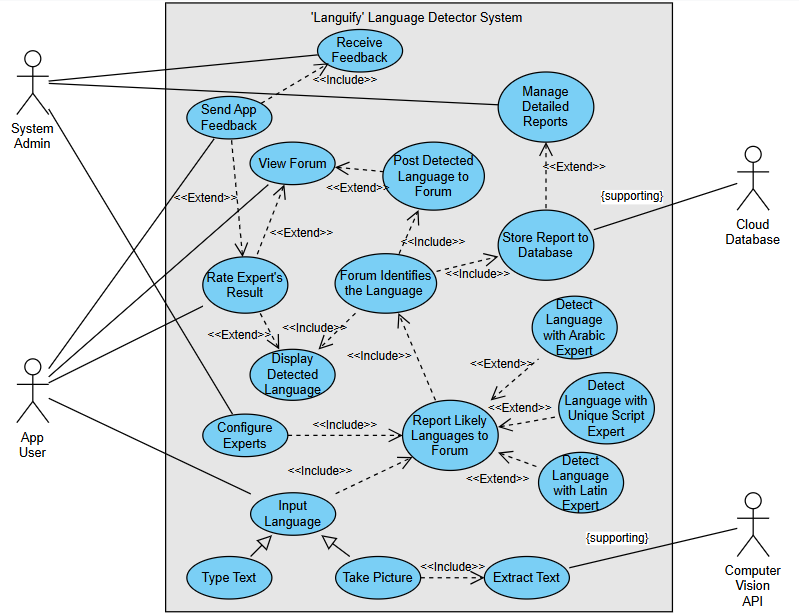
\includegraphics[width=\linewidth]{Section3/UseCaseDiagram.png}
% 	\caption{Use Case Diagram}
% 	\label{UseCaseDiagram}
% \end{figure}
\begin{figure}[H]
	\centering
	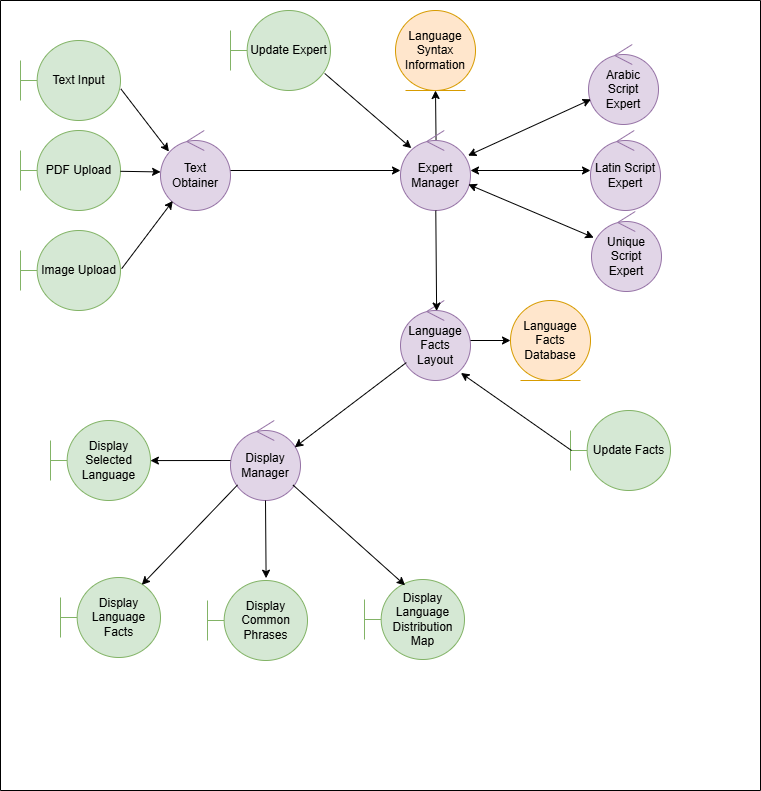
\includegraphics[width=\linewidth]{Section2/class_diagramV3.png}
	\caption{Analysis Class Diagram}
	\label{AnalysisClassDiagram}
\end{figure}


% End Section


% SECTION 3
\section{Architectural Design }
\label{sec:architectural_design}
% Begin Section

\subsection{System Architecture}
\label{sub:system_architecture}
% Begin SubSection
The overall architecture of our design follows the Pipe and Filter architecture. This serves as the overarching architecture composing of three subsystems with their own architectures, as shown in the table below.

\begin{table}[h]
    \centering
    \begin{tabularx}{\linewidth}{|X|X|X|}
        \hline
        Subsystem & Purpose & Architectural Style \\ \hline
        Reader & 
        Reads the input from the user and converts it into the
        proper file format for the 
        Identifier subsystem
        & Pipe and Filter \\ \hline
        Identifier
        &
        Identifies the language 
        using the input from the 
        Reader subsystem
        &
        Blackboard \\ \hline
        \centering Display (Facts) 
        & 
        Obtains the proper facts of 
        the identified language from 
        the Identifier subsystem 
        and displays it to the user
        & 
        Repository \\ \hline
        
    \end{tabularx}
    \caption{Architecture Table}
    \label{tab:architecture_table}
\end{table}

As data enters the system (i.e., user input), the subsystems act as filters, transforming and transferring the data through pipes to the next subsystem. A Pipe and Filter architecture consists of a data source (user input), filters (subsystems), pipes (which transfer data between subsystems), and a data sink (output to the user).
The data source pushes data only (i.e., write-only) to the Reader subsystem, which operates in a pull/push manner (i.e., read/write) by reading the input and sending it to the next subsystem, the Identifier. The Identifier subsystem also follows a pull/push model, reading data from the Reader subsystem and passing it to the Display subsystem. The Display subsystem, in turn, is pull-only (i.e., read-only), as it retrieves data from the Identifier subsystem to display the final output to the user.
In this architecture, filters are passive, while pipes are active. For a more detailed explanation of the subsystems, refer to Section 3.2.

% \begin{itemize}
%     \item Identify and explain the overall architecture of your system – Cheukman
%     \item Be sure to clearly state the name of the architecture you used (this is the name of the architectural pattern, not the name of your system) – Cheukman
%     \item Provide the reasoning and justification of the choice of architecture – Cheukman 
%     \item Provide a structural architecture diagram showing the relationship among the subsystems (if appropriate) – Gurman
    
% \end{itemize}

\begin{figure}[H]
	\centering
	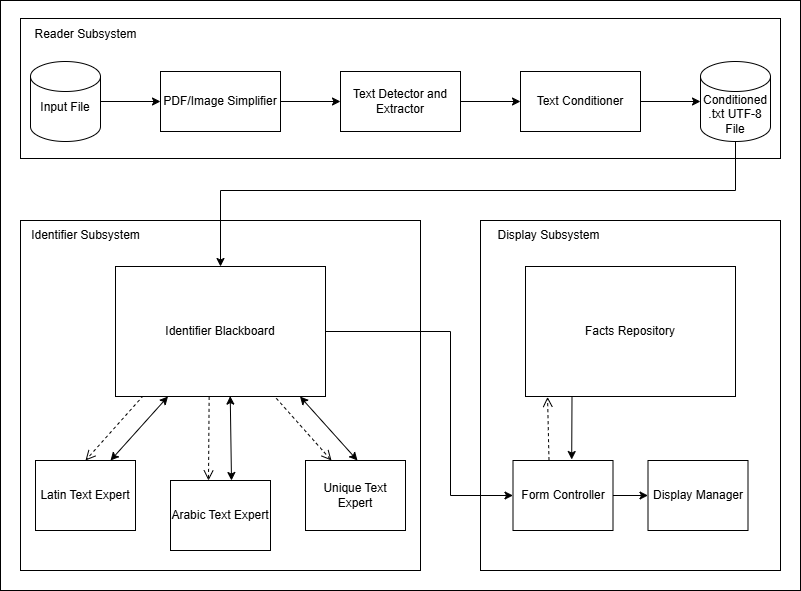
\includegraphics[width=\linewidth]{Section3/architectural_diagramV2.png}
	\caption{Architectural Diagram}
	\label{ArchitecturalDiagram}
\end{figure}

\begin{itemize}
    \item We considered Batch Sequential Architecture Style to transfer the data between different modules. However, using temporary files as connection between each module are not as efficient as Pipe and filter architecture which using data stream. The character of language could use ASCII table or UTF-8 to present. In this case, as long as the amount of data stream is not exceling pipe capacity, pipe could work more efficiently without waiting for temporary file from upstream.
    \item Master- Slave Architecture are also considered, since the slave nodes could implement experts of identifying the input language. However, Master-Slave Architecture features on divide the huge or data set into parts and process each part of task in parallel. And identify language is not a task that could divided in parts and send to the slave nodes. 
    \item We eliminate Model-View-Controller Architecture, through it have one data set that could store knowledge of different languages. However, the different view of displaying data is used for displaying what language we get instead of identifying languages. 
\end{itemize}
% End SubSection

\subsection{Subsystems}
\label{sub:subsystems}
% Begin SubSection
The system’s overall functionality is facilitated by three interconnected subsystems: the Reader, Identifier, and Display services. 
\\
\\
The purpose of the Reader service is to take some form of photo, PDF, or textual language representation, and apply the necessary transformations to convert it into a plain UTF-8 text file. This behaviour is best encapsulated by a pipe and filter architecture, as the different input types dictate how they will be sequentially filtered. This can be done very efficiently over a data stream as each of the accepted file formats are static types, making them easy to binarize. Also, since users only submit a few (between 1-5) supplementary files per request, handling each one individually incurs less latency and wasted resources than using a batch sequential alternative. Data flow architectures often suffer due to their low throughputs; however, since all input processing occurs on a user’s local device, each request is managed by its own processor, and this is not an issue. These characteristics make the pipe and filter architecture ideal for the Reader service.
\\
\\
The Identifier service takes the normalized UTF-8 text provided by the Reader service, and interprets what language it is written in. To do this, it makes use of the blackboard architecture. This way, when the input arrives at the data store, it can call upon its agents (knowledge sources) to analyze the input and guess the language. More agents can be added down the line, allowing for more accurate deductions. There is no way for the agents to be certain about the language, but each offers partial solutions that build towards a comprehensive estimate. Therefore, the Identifier service’s need for an active data store and knowledge source is best fulfilled by a blackboard architecture.  
\\
\\
The third main subsystem is the Display service, which stores and returns all the interesting statistics, words, and phrases to be displayed upon language detection. As its duty is simply to store information so it can be retrieved by other agents, the repository architecture is best to implement it. The Identifier system acts as an active agent in this case by making requests for information in the passive data store. This rules out a blackboard architecture since it would need an active data store and provides uncertain partial solutions, which is not what this situation demands. The repository architecture also helps with scalability as this information is likely to be stored on a server, so when there are many concurrent requests, they all access the same network. The repository architecture is adept at handling this traffic as each one may be interpreted as a different agent, whereas a data flow architecture would have to process them one at a time, bottlenecking the system. To maintain a responsive application, the repository architecture works best for the display service. 
\\
\\
In general, the Reader service acts as a bootstrap for the blackboard identifier, and once it computes the language, the display subsystem assists it in projecting a comprehensive output to the user. 
% End SubSection


% SECTION 4
\section{Class Responsibility Collaboration (CRC) Cards}
\label{sec:crc_cards}
% Begin Section

% \input{Section4/card1}
\begin{cards}[]
    \textbf{Class Name:} Text Obtainer (Controller)
    % \medskip % Adds spacing
    % \noindent\rule{\linewidth}{0.4pt} % Full-width horizontal line
    % \medskip
    \tcbline
    \begin{tabular}{p{0.45\linewidth} | p{0.45\linewidth}}
        \textbf{Responsibility:}& 
        \textbf{Collaborator:}\\
        % \hline % Horizontal line inside the table
    \end{tabular}
    \tcbline
    \begin{tabular}{p{0.45\linewidth} | p{0.45\linewidth}}
        \begin{itemize}
            \item Knows Text Input
            \item Knows PDF Upload
            \item Knows Image Upload
            \item Knows Expert Manager
            \item Knows how to extract text from PDF files and Images
            \item Knows how to convert text to UTF-8 file
 
        \end{itemize}
        &
        \begin{itemize}
            \item Text Input
            \item PDF Upload
            \item Image Upload
            \item Expert Manager
             
        \end{itemize}
    \end{tabular}
\end{cards}
\begin{cards}[]
    \textbf{Class Name:} Text Input (Boundary)
    % \medskip % Adds spacing
    % \noindent\rule{\linewidth}{0.4pt} % Full-width horizontal line
    % \medskip
    \tcbline
    \begin{tabular}{p{0.45\linewidth} | p{0.45\linewidth}}
        \textbf{Responsibility:}& 
        \textbf{Collaborator:}\\
        % \hline % Horizontal line inside the table
    \end{tabular}
    \tcbline
    \begin{tabular}{p{0.45\linewidth} | p{0.45\linewidth}}
        \begin{itemize}
            \item Handles event of entering typed input
            \item Sends this typed input to Text Obtainer
            
        \end{itemize}
        &
        \begin{itemize}
            \item Text Obtainer
        \end{itemize}
    \end{tabular}
\end{cards}
\begin{cards}[]
    \textbf{Class Name:} PDF Upload (Boundary)
    % \medskip % Adds spacing
    % \noindent\rule{\linewidth}{0.4pt} % Full-width horizontal line
    % \medskip
    \tcbline
    \begin{tabular}{p{0.45\linewidth} | p{0.45\linewidth}}
        \textbf{Responsibility:}& 
        \textbf{Collaborator:}\\
        % \hline % Horizontal line inside the table
    \end{tabular}
    \tcbline
    \begin{tabular}{p{0.45\linewidth} | p{0.45\linewidth}}
        \begin{itemize}
            \item Handles event of uploading PDF
            \item Sends this PDF to Text Obtainer
        \end{itemize}
        &
        \begin{itemize}
            \item Text Obtainer
        \end{itemize}
    \end{tabular}
\end{cards}
\begin{cards}[]
    \textbf{Class Name:} Image Upload (Boundary)
    % \medskip % Adds spacing
    % \noindent\rule{\linewidth}{0.4pt} % Full-width horizontal line
    % \medskip
    \tcbline
    \begin{tabular}{p{0.45\linewidth} | p{0.45\linewidth}}
        \textbf{Responsibility:}& 
        \textbf{Collaborator:}\\
        % \hline % Horizontal line inside the table
    \end{tabular}
    \tcbline
    \begin{tabular}{p{0.45\linewidth} | p{0.45\linewidth}}
        \begin{itemize}
            \item Handles event of uploading image
            \item Sends this image to Text Obtainer
            \item \textcolor{red}{Knows Text Obtainer}
        \end{itemize}
        &
        \begin{itemize}
            \item Text Obtainer
        \end{itemize}
    \end{tabular}
\end{cards}
\begin{cards}[]
    \textbf{Class Name:} Expert Manager (Controller)
    % \medskip % Adds spacing
    % \noindent\rule{\linewidth}{0.4pt} % Full-width horizontal line
    % \medskip
    \tcbline
    \begin{tabular}{p{0.45\linewidth} | p{0.45\linewidth}}
        \textbf{Responsibility:}& 
        \textbf{Collaborator:}\\
        % \hline % Horizontal line inside the table
    \end{tabular}
    \tcbline
    \begin{tabular}{p{0.45\linewidth} | p{0.45\linewidth}}
        \begin{itemize}
            \item Knows Update Expert
            \item Knows Language Syntax Information
            \item Communicates with Arabic Script Expert, Latin Script Expert, Unique Script Expert
            
        \end{itemize}
        &
        \begin{itemize}
            \item Update Expert
            \item Language Syntax Information
            \item Arabic Script Expert
            \item Latin Script Expert
            \item Unique Script Expert
            
        \end{itemize}
    \end{tabular}
\end{cards}
\begin{cards}[]
    \textbf{Class Name:} Update Expert (Boundary)
    % \medskip % Adds spacing
    % \noindent\rule{\linewidth}{0.4pt} % Full-width horizontal line
    % \medskip
    \tcbline
    \begin{tabular}{p{0.45\linewidth} | p{0.45\linewidth}}
        \textbf{Responsibility:}& 
        \textbf{Collaborator:}\\
        % \hline % Horizontal line inside the table
    \end{tabular}
    \tcbline
    \begin{tabular}{p{0.45\linewidth} | p{0.45\linewidth}}
        \begin{itemize}
            \item Handles event of add expert
            \item Handles event of edit expert
            \item Handles event of delete expert
            \item Knows Expert Manager
            \item \textcolor{red}{Knows Admin Console}
        \end{itemize}
        &
        \begin{itemize}
            \item \textcolor{red}{Admin Console}
        \end{itemize}
    \end{tabular}
\end{cards}
\begin{cards}[]
    \textbf{Class Name:} Language Syntax Information (Entity)
    % \medskip % Adds spacing
    % \noindent\rule{\linewidth}{0.4pt} % Full-width horizontal line
    % \medskip
    \tcbline
    \begin{tabular}{p{0.45\linewidth} | p{0.45\linewidth}}
        \textbf{Responsibility:}& 
        \textbf{Collaborator:}\\
        % \hline % Horizontal line inside the table
    \end{tabular}
    \tcbline
    \begin{tabular}{p{0.45\linewidth} | p{0.45\linewidth}}
        \begin{itemize}
            \item Knows Detectable Languages
            \item Knows Syntax for every Detectable Language
            \item \textcolor{red}{Knows Expert Manager}
        \end{itemize}
        &
        \begin{itemize}
            \item Expert Manager
        \end{itemize}
    \end{tabular}
\end{cards}
\begin{cards}[]
    \textbf{Class Name:} Arabic Script Expert (Controller)
    % \medskip % Adds spacing
    % \noindent\rule{\linewidth}{0.4pt} % Full-width horizontal line
    % \medskip
    \tcbline
    \begin{tabular}{p{0.45\linewidth} | p{0.45\linewidth}}
        \textbf{Responsibility:}& 
        \textbf{Collaborator:}\\
        % \hline % Horizontal line inside the table
    \end{tabular}
    \tcbline
    \begin{tabular}{p{0.45\linewidth} | p{0.45\linewidth}}
        \begin{itemize}
            \item Give vital language identification information to the Expert manager
        \end{itemize}
        &
        \begin{itemize}
            \item Expert Manager
        \end{itemize}
    \end{tabular}
\end{cards}
\begin{cards}[]
    \textbf{Class Name:} Latin Script Expert (Controller)
    % \medskip % Adds spacing
    % \noindent\rule{\linewidth}{0.4pt} % Full-width horizontal line
    % \medskip
    \tcbline
    \begin{tabular}{p{0.45\linewidth} | p{0.45\linewidth}}
        \textbf{Responsibility:}& 
        \textbf{Collaborator:}\\
        % \hline % Horizontal line inside the table
    \end{tabular}
    \tcbline
    \begin{tabular}{p{0.45\linewidth} | p{0.45\linewidth}}
        \begin{itemize}
            \item Give vital language identification information to the Expert manager
        \end{itemize}
        &
        \begin{itemize}
            \item Expert Manager
        \end{itemize}
    \end{tabular}
\end{cards}
\begin{cards}[]
    \textbf{Class Name:} Unique Script Expert (Controller)
    % \medskip % Adds spacing
    % \noindent\rule{\linewidth}{0.4pt} % Full-width horizontal line
    % \medskip
    \tcbline
    \begin{tabular}{p{0.45\linewidth} | p{0.45\linewidth}}
        \textbf{Responsibility:}& 
        \textbf{Collaborator:}\\
        % \hline % Horizontal line inside the table
    \end{tabular}
    \tcbline
    \begin{tabular}{p{0.45\linewidth} | p{0.45\linewidth}}
        \begin{itemize}
            \item Give vital language identification information to the Expert manager
        \end{itemize}
        &
        \begin{itemize}
            \item Expert Manager
        \end{itemize}
    \end{tabular}
\end{cards}
\begin{cards}[]
    \textbf{Class Name:} Language Facts Layout (Controller)
    % \medskip % Adds spacing
    % \noindent\rule{\linewidth}{0.4pt} % Full-width horizontal line
    % \medskip
    \tcbline
    \begin{tabular}{p{0.45\linewidth} | p{0.45\linewidth}}
        \textbf{Responsibility:}& 
        \textbf{Collaborator:}\\
        % \hline % Horizontal line inside the table
    \end{tabular}
    \tcbline
    \begin{tabular}{p{0.45\linewidth} | p{0.45\linewidth}}
        \begin{itemize}
            \item Handles information sent from the Expert Manager
            \item Accesses Language Facts Database
            % \item Accepts input from Updated facts and updates the Language Facts Database
            \item \textcolor{red}{Updates the Language Facts Database signaled by Admin Console}
            \item Sends information pertaining to form control to the Display Manager
             
        \end{itemize}
        &
        \begin{itemize}
            \item Display Manager
            \item Language Facts Database
            \item Expert Manager
            \item \textcolor{red}{Admin Console}
            % \item Update Facts
            
        \end{itemize}
    \end{tabular}
\end{cards}
\begin{cards}[]
    \textbf{Class Name:} Language Facts Database (Entity)
    % \medskip % Adds spacing
    % \noindent\rule{\linewidth}{0.4pt} % Full-width horizontal line
    % \medskip
    \tcbline
    \begin{tabular}{p{0.45\linewidth} | p{0.45\linewidth}}
        \textbf{Responsibility:}& 
        \textbf{Collaborator:}\\
        % \hline % Horizontal line inside the table
    \end{tabular}
    \tcbline
    \begin{tabular}{p{0.45\linewidth} | p{0.45\linewidth}}
        \begin{itemize}
            \item A database that stores facts that corresponded to identified language.
            \item \textcolor{red}{Knows Language Facts Layout}
        \end{itemize}
        &
        \begin{itemize}
            \item Language Facts Layout
        \end{itemize}
    \end{tabular}
\end{cards}
\newpage
\begin{cards}[]
    \textbf{Class Name:} Update Facts (Boundary)
    % \medskip % Adds spacing
    % \noindent\rule{\linewidth}{0.4pt} % Full-width horizontal line
    % \medskip
    \tcbline
    \begin{tabular}{p{0.45\linewidth} | p{0.45\linewidth}}
        \textbf{Responsibility:}& 
        \textbf{Collaborator:}\\
        % \hline % Horizontal line inside the table
    \end{tabular}
    \tcbline
    \begin{tabular}{p{0.45\linewidth} | p{0.45\linewidth}}
        \begin{itemize}
            \item Gives vital language identification information to the Expert manager
            \item Knows Language Facts Layout Controller
            \item Handle update facts of different languages
            \item \textcolor{red}{Knows Admin Console}
        \end{itemize}
        &
        \begin{itemize}
            \item \textcolor{red}{Admin Console}
        \end{itemize}
    \end{tabular}
\end{cards}
\begin{cards}[]
    \textbf{Class Name:} Display Manager (Controller)
    % \medskip % Adds spacing
    % \noindent\rule{\linewidth}{0.4pt} % Full-width horizontal line
    % \medskip
    \tcbline
    \begin{tabular}{p{0.45\linewidth} | p{0.45\linewidth}}
        \textbf{Responsibility:}& 
        \textbf{Collaborator:}\\
        % \hline % Horizontal line inside the table
    \end{tabular}
    \tcbline
    \begin{tabular}{p{0.45\linewidth} | p{0.45\linewidth}}
        \begin{itemize}
            \item Handles information sent from the Language Facts Layout Controller
            \item Send Information to Display language fact
            \item Send result of language to Display selected language
            \item Send information to language common phrases
            \item Send information to Display map of language spread
            
        \end{itemize}
        &
        \begin{itemize}
            \item Language Facts Layout
            \item Display Language Facts
            \item Display Selected Language
            \item Display Common Phrases
            \item Display Language Distribution Map

        \end{itemize}
    \end{tabular}
\end{cards}
\begin{cards}[]
    \textbf{Class Name:} Display Selected Language (Boundary)
    % \medskip % Adds spacing
    % \noindent\rule{\linewidth}{0.4pt} % Full-width horizontal line
    % \medskip
    \tcbline
    \begin{tabular}{p{0.45\linewidth} | p{0.45\linewidth}}
        \textbf{Responsibility:}& 
        \textbf{Collaborator:}\\
        % \hline % Horizontal line inside the table
    \end{tabular}
    \tcbline
    \begin{tabular}{p{0.45\linewidth} | p{0.45\linewidth}}
        \begin{itemize}
            \item Displays the language selected
        \end{itemize}
        &
        \begin{itemize}
            \item Display Manager
        \end{itemize}
    \end{tabular}
\end{cards}
\begin{cards}[]
    \textbf{Class Name:} Display Language Facts (Boundary)
    % \medskip % Adds spacing
    % \noindent\rule{\linewidth}{0.4pt} % Full-width horizontal line
    % \medskip
    \tcbline
    \begin{tabular}{p{0.45\linewidth} | p{0.45\linewidth}}
        \textbf{Responsibility:}& 
        \textbf{Collaborator:}\\
        % \hline % Horizontal line inside the table
    \end{tabular}
    \tcbline
    \begin{tabular}{p{0.45\linewidth} | p{0.45\linewidth}}
        \begin{itemize}
            \item Displays language facts to the user, such as number of speakers
        \end{itemize}
        &
        \begin{itemize}
            \item Display Manager
        \end{itemize}
    \end{tabular}
\end{cards}
\begin{cards}[]
    \textbf{Class Name:} Display Common Phrases (Boundary)
    % \medskip % Adds spacing
    % \noindent\rule{\linewidth}{0.4pt} % Full-width horizontal line
    % \medskip
    \tcbline
    \begin{tabular}{p{0.45\linewidth} | p{0.45\linewidth}}
        \textbf{Responsibility:}& 
        \textbf{Collaborator:}\\
        % \hline % Horizontal line inside the table
    \end{tabular}
    \tcbline
    \begin{tabular}{p{0.45\linewidth} | p{0.45\linewidth}}
        \begin{itemize}
            \item Displays a list of common phrases from the selected language
        \end{itemize}
        &
        \begin{itemize}
            \item Display Manager
        \end{itemize}
    \end{tabular}
\end{cards}
\begin{cards}[]
    \textbf{Class Name:} Display Language Distribution Map (Boundary)
    % \medskip % Adds spacing
    % \noindent\rule{\linewidth}{0.4pt} % Full-width horizontal line
    % \medskip
    \tcbline
    \begin{tabular}{p{0.45\linewidth} | p{0.45\linewidth}}
        \textbf{Responsibility:}& 
        \textbf{Collaborator:}\\
        % \hline % Horizontal line inside the table
    \end{tabular}
    \tcbline
    \begin{tabular}{p{0.45\linewidth} | p{0.45\linewidth}}
        \begin{itemize}
            \item Displays a diagram showcasing where the language is spoken
        \end{itemize}
        &
        \begin{itemize}
            \item Display Manager
        \end{itemize}
    \end{tabular}
\end{cards}



% DIVISION OF LABOR
\appendix
\section{Division of Labour}
\label{sec:division_of_labour}
% Begin Section

\textbf{Andy Huynh}
\begin{itemize}
    \item Worked on Section 4 Business Events with Ke Ma
    \item Set up and translated all the text into the LaTeX file
    \item Worked on Sections 5.5, 5.6, and 5.7 with Ke Ma
\end{itemize}
\begin{figure}[H]
	\centering
	
\includegraphics[width=0.2\textwidth]{Signatures/a.png}  
\end{figure}

\textbf{Cheukman Zhou}
\begin{itemize}
    \item Worked on Section 1.2
    \item Worked on Section 3.1
    \item Helped with formatting and editing of the document on LaTeX
\end{itemize}
\begin{figure}[H]
	\centering
	
\includegraphics[width=0.2\textwidth]{Signatures/c.png}
\end{figure}

\textbf{Ke Ma}
\begin{itemize}
    \item Worked on Section 4 with Andy Huynh
    \item Worked on Sections 5.5, 5.6, and 5.7 with Andy Huynh
\end{itemize}
\begin{figure}[H]
	\centering
	
\includegraphics[width=0.2\textwidth]{Signatures/k.png}
\end{figure}

\textbf{Sarah Dorfman}
\begin{itemize}
    \item Worked on Section 2 alongside Cheukman Zhou
    \item Worked on Section 5.1
\end{itemize}
\begin{figure}[H]
	\centering
	
\includegraphics[width=0.2\textwidth]{Signatures/s.png}
\end{figure}

\textbf{Gurmanjot Minhas}
\begin{itemize}
    \item Worked on Section 3
    \item Worked on Sections 5.4 and 5.8
    \item Completed Section 6: Innovative Ideas
\end{itemize}
\begin{figure}[H]
	\centering
	
\includegraphics[width=0.2\textwidth]{Signatures/g.png}
\end{figure}

% End Section


\end{document}
%------------------------------------------------------------------------------